\documentclass[11pt,letterpaper,fleqn]{report}
\usepackage{amsmath,amsthm,amsfonts,amssymb,amscd}
\usepackage{fullpage}
\usepackage{lastpage}
\usepackage{enumerate}
\usepackage{fancyhdr}
\usepackage[percent]{overpic}
\usepackage{mathrsfs}
\usepackage{wrapfig}
\usepackage{multirow}
\usepackage{amsmath}
\usepackage{amssymb}
\usepackage{amscd}
\usepackage{placeins}
\usepackage{lscape}
\usepackage{graphicx}
\usepackage[usenames,dvipsnames]{color}
\usepackage{listings}
\usepackage[usenames,dvipsnames,svgnames,table]{xcolor}
\usepackage[left=2.5cm,right=2.5cm,top=2.5cm,bottom=2.5cm, headsep = 0.9cm]{geometry}
\usepackage{verbdef}
\setlength{\parindent}{0.0in}
\setlength{\parskip}{0.0in}
\usepackage{setspace}
\definecolor{gray}{RGB}{90,90,90}
\usepackage[colorlinks=true, linktoc=all, linkcolor=blue]{hyperref}

\pagestyle{plain}

\begin{document}
\centerline{\textbf{\Large{An Introduction to R}}}
\centerline{\textbf{Authors: Andrew J. Spieker and Brian D. Williamson}}
\tableofcontents

\chapter{Introduction}
This document is meant for students to get an introductory look at R (and how it compares to and differs from STATA), and to facilitate a transition for both students and instructors from STATA to R, using both the base R functions and the \texttt{uwIntroStats} package developed by Scott S. Emerson, M.D. Ph.D., Andrew J. Spieker, and Brian D. Williamson in the University of Washington Department of Biostatistics.

R is a functional language at the basic level, meaning that even the simple expression \texttt{3 + 5} is handed to a function called \texttt{evaluate()}, which then returns the result. Most objects and functions have a print function, so we can either print and display results or store them as an object. STATA, on the other hand, is a command style language. The user types in a command and the result is displayed. In this file we will present some of the useful R functions, but there are many more that we leave to the reader to go out and find. Also, even if we do present a function here, we will be doing so at the most basic level. Many of the functions have more capabilities than what we show.

\chapter{Project Management}
\section{The Workspace}
There are a few differences between R and STATA when it comes to data and project management. The first concept that we must cover is that of the workspace. In STATA, you are only allowed to read in one data set at a time. This data set is your entire workspace, and thus all functions and calls manipulate the data set. In R, however, the workspace consists of many different data sets, values, and functions. Any variable that is assigned a name becomes part of the workspace. Upon exit from R, the program asks the user if they wish to save the workspace. Saying yes saves all variables, functions, and data sets and then loads them back in to the workspace upon startup of the program the next time. It is generally good practice to save the workspace, especially if you know that you will continue to work with the same data next time.

To start, we will assume you are running R from the command line. Later on, if you wish, we will introduce a convenient graphical user interface. However, it is good to learn the basics from the command line and know what is happening behind the buttons in the GUI. Once you navigate to the correct directory for R (in a Windows machine this is generally in ``C:\textbackslash Program Files\textbackslash R\textbackslash R-version\textbackslash bin'' - substitue the version of R you downloaded for ``version''), you simply type ``R'' and the program will start, displaying a screen similar to this:

\begin{figure}[h!]
\centering
	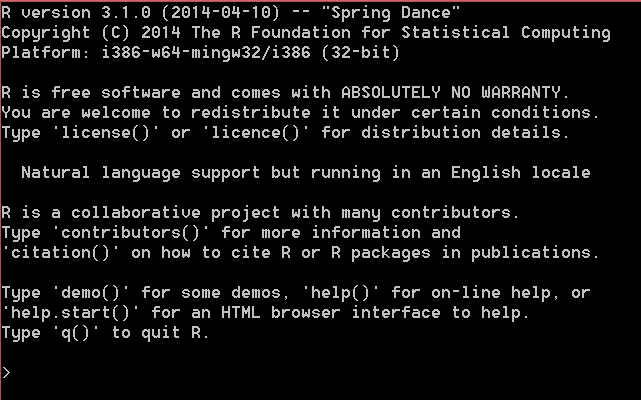
\includegraphics[width=5in]{r_welcome.png}
\end{figure}

If you type `q()', you are prompted to \texttt{Save workspace image? [y/n/c]: }, where `\texttt{y}' is yes, `\texttt{n}' is no, and `\texttt{c}' is cancel. If you type `\texttt{y}', then two files are created: a \texttt{.Rhistory} file and a \texttt{.RData} file. You can load the \texttt{.RData} file at the beginning of a session with the \texttt{load()} function, and it brings in all of your variables, data sets, and functions. The \texttt{.Rhistory} file saves all of your commands from the session. If you are working with a few different projects, it is a good idea to have a workspace for each of these projects. Then any one workspace doesn't get too cluttered.
\section{Scripts}
Scripts are useful files that can be run by R. A script file can be created in any directory on your computer. Then it can be ``sourced'', using the \texttt{source()} function (given the file path) to run all of the functions saved in the script file. A script is a useful place to write all of your function calls so that you can save them for later. For example, on a Windows computer, we could create a script file on the Desktop by using any text editor (Notepad or any other that you prefer) and saving the file with the \texttt{.R} extension, such as:
\begin{verbatim}
test_script.R
\end{verbatim}
We can then load all of the functions and run all of the code saved in the script by opening R and typing (recall that our script file is located on the desktop)
\begin{verbatim}
source(``C://Users//Brian Williamson//Desktop//test_script.R'')
\end{verbatim}
\section{Comments}
Commenting your files is always a good idea. Comments provide information as to why you are using certain functions at certain times. The comment key in R is \texttt{\#}. If you type this at any point on a line, the rest of the line will not be run by R.

\chapter{Data}

\section{Data Types (`storage.mode')}
A huge reason for using R at all is its data capabilities. There are many types of data in R, and thus it is important to know what kind of data you are dealing with at a given time. The ``\texttt{storage.mode()}'' function returns what type the data is. The basic data types are:

\subsection{Numeric}
Decimal values are numerics. Numeric is the default computational data type in R. \emph{Note for the curious: all real numbers in R are stored as ``doubles'', meaning that the IEEE floating point number is stored as a 64 bit word rather than a 32 bit word.} There are two subtypes of numeric values. Most of the time there is no need to worry about the difference between them, but every once in a while you need to know which type you are dealing with.

\textbf{Integer}\\
A whole number. 
\newline \textbf{Double}\\
A real number (whole number plus fractional part).

\subsection{Character}
A character is an object which represents string values. For example, "3" is a character. To convert an object into a character, use the \texttt{as.character()} function. 

\subsection{Logical}
\texttt{TRUE} and \texttt{FALSE} are the logical values in R, usually produced by comparisons. The standard logical operators in R are: 
\begin{tabular}{ll}
``\&"  & and \\
``$\mid$" & or \\
``!" & negation\\
``==" & equals
\end{tabular}

\subsection{NA, NULL, Inf, and NaN}
\texttt{NA} denotes a missing value in R. \texttt{NA} is a logical constant of length 1.

\texttt{NULL} is the null object in R. Functions and expressions whose values are undefined sometimes return \texttt{NULL}. If a \texttt{NULL} value is compared to another (for example, \texttt{NULL == 0}), then the result will be the expression \texttt{logical(0)}. The length of the \texttt{NULL} object is 0.\\
\texttt{Inf} is returned by dividing any number besides 0 by 0.\\
\texttt{NaN} (not a number) is returned by the expression dividing 0 by 0.

\begin{verbatim}
0/0
[1] NaN
1/0
[1] Inf
\end{verbatim}

\subsection{Factor}
A factor stores the nominal values of the data (starting with 1) in a vector, and stores the associated names of the data as a vector of character strings. A factor is created with the \texttt{factor()} function. For example, let's say that we have a vector with twenty \texttt{``male''}'s and twenty \texttt{``female''}'s. Then a factor would store this data as twenty 1s and twenty 2s, and would have a key telling us that \texttt{1} was male and \texttt{2} was female. \emph{For the really curious: factors are really data structures, since they are a vector with attributes.}
%\subsubsection{Complex}
%A complex number - has an imaginary component.

\section{Data Structures}
There are a variety of data structures in R. They include vectors, matrices, arrays, data frames, lists, and factors.

\subsection{Vectors}
A vector is the most simple data structure in R. A vector stores any number of individual values, but they must be all of the same type. A vector is created with the \texttt{c()} function.

\subsection{Matrices}
A matrix is a table, is essentially a two-dimensional vector. All values in the matrix must be of the same data type, and a matrix must be rectangular - that is, each row must have the same number of columns as the others and each column must have the same number of rows as the others. A matrix is created with the \texttt{matrix()} function. 

\subsection{Arrays}
An array is a high-dimensional matrix. An array is created with the \texttt{array} function.

\subsection{Data frame}
A data frame is a table, like a matrix. However, the columns in a data frame may have different data types. A data frame is created with the \texttt{data.frame()} function.

\subsection{List}
A list is an ordered collection of objects. The values in a list can be any data type or data structure, and they don't have to have the same size. A list is created with the \texttt{list()} function. \emph{A note for the curious: lists indirectly reference their values. They are stored in different places in memory as addresses.} Lists are sometimes returned from functions.

\section{Assigning a Value to a Variable}
Let's say we want to creat a variable called \texttt{junk}. Then we must assign \texttt{junk} a value. Here we will assign it the number \texttt{1}. Thus, we type 
\begin{verbatim}
junk <- 1
\end{verbatim}
And now any time that we wish to see what \texttt{junk} is, we type \texttt{junk} and get the output 
\begin{verbatim}
junk
[1] 1
\end{verbatim}
Any time we wish to assign a value to a variable, we use the ``\texttt{<-}'' function. This guarantees that we perform the correct assignment (some functions and packages were developed in a time where using ``='' as assignment will not work correctly).

\section{Returning a Value from a Data Structure}
There are three main ways of accessing data in a data set. The main ways deal with data sets in vector or matrix form (similar syntax), list form, or data frame form. 

\subsection{The ``[ ]'' Operator}
The first way we will cover is for vectors and matrices. Let's say we have a vector representing the numbers 1-10. This vector can be stored as \begin{verbatim}> test <- c(1,2,3,4,5,6,7,8,9,10) \end{verbatim} Now if we wish to access the 6, we type 
\begin{verbatim}
test[6] 
\end{verbatim}
Which returns
\begin{verbatim}
[1] 6
\end{verbatim} 
Recall that R is a functional language at its base. Thus, if we want to see the sixth value of \texttt{test}, we can type in any expression which will evaluate to 6. For example:
\begin{verbatim}
test[3+3]
[1] 6
\end{verbatim}
Now, a vector is simply a matrix with one row. Thus let's consider a matrix with 735 rows and 30 columns (we will be using this matrix later as well) called \texttt{mri}. If we wish to access an entry in the matrix we type in the row and column of interest: 
\begin{verbatim}
mri[1,1]
[1] 1
\end{verbatim}
Which returns the value in row 1, column 1 as we requested.

\subsection{The ``\$'' Operator}
A data frame, as we discussed earlier, is a list of vectors. Let's use the \texttt{mriTest} data frame that we created earlier. Now we can access a value from the data frame either by the \texttt{[rownum,colnum]} or \texttt{[rownum,"colname"]} function or by the \texttt{\$colname[rownum]} function:
\begin{verbatim}
mriTest[1,1]
[1] 1 
mriTest[1,"ptid"]
[1] 1 
mriTest$ptid[1]
[1] 1 
\end{verbatim}

\section{Indexing Values in a Data Structure}
Sometimes, it is useful to access more than one value from a data structure. 

\subsection{The ``[ ]'' operator}
If we want to see the first five elements of the vector, we type
\begin{verbatim}
test[1:5]
\end{verbatim}
which returns
\begin{verbatim}
[1] 1 2 3 4 5 
\end{verbatim}
Now recall the \texttt{mri} data set. If we wish to access the entire first row (a vector!) we type 
\begin{verbatim}
mri[1,]
\end{verbatim}
Which means that we are selecting the first row and all of the columns. The \texttt{[row,column]} format is followed for matrices. The output of this call is 
\begin{verbatim}
  ptid mridate age male race weight height packyrs yrsquit alcoh physact chf chd
1    1  120791  72    1    2    173    169      54       0     0    9.84   0   1
  stroke diabetes genhlth ldl alb crt plt sbp    aai   fev dsst atrophy whgrd
1      2        0       3 135 3.7 1.4 275 139 1.0303 1.284   25      20     2
  numinf volinf obstime death
1      1 7.4613    2110     0
\end{verbatim}

\subsection{Special Issues for Indexing a Matrix}
However, when we are subscripting a matrix, we may wish to be sure what class our returned value is. For example, a test matrix
\begin{verbatim}
m <- matrix(rep(1, 30), nrow=3)
m
     [,1] [,2] [,3] [,4] [,5] [,6] [,7] [,8] [,9] [,10]
[1,]    1    1    1    1    1    1    1    1    1     1
[2,]    1    1    1    1    1    1    1    1    1     1
[3,]    1    1    1    1    1    1    1    1    1     1
\end{verbatim}
If we want the first row of the matrix, and want it to be a matrix, we will run into problems if we simply type \texttt{m[1,]}. 
\begin{verbatim}
m[1,]
 [1] 1 1 1 1 1 1 1 1 1 1
\end{verbatim}
Notice that this returned a vector! If we want a matrix, we must type
\begin{verbatim}
m[1,,drop=FALSE]
     [,1] [,2] [,3] [,4] [,5] [,6] [,7] [,8] [,9] [,10]
[1,]    1    1    1    1    1    1    1    1    1     1
\end{verbatim}
Adding the \texttt{drop=FALSE} argument after our row and column specifications told R not to drop dimensions and create a vector.
\subsection{The ``\$'' Operator}
Let's use the \texttt{mriTest} data frame that we created earlier. Now we can access a column of the data frame either by the \texttt{[,colnum]} or \texttt{[,"colname"]} function or by the \texttt{\$colname} function, as we see here (we only get the first three rows to save paper):
\begin{verbatim}
mriTest[1:3,1]
[1] 1 2 3
mriTest[1:3,"ptid"]
[1] 1 2 3
mriTest$ptid[1:3]
[1] 1 2 3
\end{verbatim}
Last, variables in matrices, lists, and data frames can both be accessed using the \texttt{\$} operator. Create \texttt{sampleList} to have a vector of strings, a matrix, and a single number as follows:
\begin{verbatim}
sampleList <- list(c("One", "Two", "Three"), mri, 1)
\end{verbatim}
Now we wish to name the elements of \texttt{sampleList}:
\begin{verbatim}
names(sampleList) <- c("strings", "matrix", "number")
\end{verbatim}
Now we can access the vector of strings either with the \texttt{[[1]]} function or with the \texttt{\$strings} function, as we can see here:
\begin{verbatim}
sampleList[[1]]
[1] "One"   "Two"   "Three"
sampleList$strings
[1] "One"   "Two"   "Three"
\end{verbatim}
\subsection{The ``[[ ]]'' Operator}
In a list, we use the \texttt{[[ ]]} operator to access elements of the list. For example, if \texttt{sampleList} is a list, then \texttt{sampleList[[1]]} returns the first element in \texttt{sampleList}. Each individual element in a list can be a different type. Thus we can have a list where the first element is a vector of strings, the second element is a matrix, and the third element is a single number. 
\section{Advanced Indexing}
\subsection{Indexing with a Vector}
Say we wish to access columns 3, 5, and 30 from \texttt{mri}, along with the first five rows. Then we use a vector to access these columns:
\begin{verbatim}
mri[1:3, c(3,5,30)]
  age race death
1  72    2     0
2  81    2     0
3  90    2     0
\end{verbatim}
We can accomplish the same thing by using the names of the columns, in \texttt{mri[1:3, c("age", "race", "death")]}.
\subsection{Indexing with a Negative Number}
Recall our vector \texttt{test}, which has ten values. If we want all of the values of test but the first, rather than indexing with the sequence \texttt{2:10}, we can simply write:
\begin{verbatim}
test[-1]
[1]  2  3  4  5  6  7  8  9 10
\end{verbatim}
We can do the same thing in a matrix - if we write \texttt{mri[-1,-1]}, R will print the whole matrix minus the first row and the first column.
\subsection{Indexing using Logicals}
Sometimes we wish to exclude values in the data based on some logical comparison. For example, in \texttt{mri}, we might to only see the values for females, or we wish to only see the values in \texttt{test} which are greater than 5. We accomplish this by using logical comparisons in our indexing. To get the values in \texttt{test} which are greater than 5, we type
\begin{verbatim}
test[test > 5]
[1]  6  7  8  9 10
\end{verbatim}
To get only the females in \texttt{mri} (and all of the columns) we type \texttt{mri[mri[,"male"] == 0,]}.
\subsection{Indexing with a Matrix}
If we have a matrix (say \texttt{mri}) and we wish to reference certain cells, we can use a matrix as a reference. The reference matrix has two columns, the first corresponding to the row of the cell in question and the second corresponding to the column of the cell in question. So if we are interested in seeing cells \texttt{[1,1]}, \texttt{[2,2]}, and \texttt{[3,3]}, we create this matrix:
\begin{verbatim}
ref <- matrix(c(1,1,2,2,3,3), ncol=2, byrow=TRUE)
ref
     [,1] [,2]
[1,]    1    1
[2,]    2    2
[3,]    3    3
\end{verbatim}
Notice that when we create a matrix, we can specify how many columns (or rows) we want with the \texttt{ncol} (\texttt{nrow}) argument, and we can specify how the matrix is filled in with the \texttt{byrow} argument. Now we use \texttt{ref} to reference these cells of \texttt{mri}
\begin{verbatim}
mri[ref]
[1]     1 90192    90
mri[1,1]
[1] 1
mri[2,2]
[1] 90192
mri[3,3]
[1] 90
\end{verbatim} 
Notice that using \texttt{ref} has returned the same values as indexing each cell individually!
\chapter{Data Input}
\section{Entering from the Keyboard}
We can enter data from the keyboard as we have done before (for example \texttt{test <- 1:10}), or we can create a data frame or some other data structure and edit using R's built in spreadsheet editor. 
\begin{verbatim}
# create a data frame
newdata <- matrix()
# bring up the spreadsheet editor and save changes into newdata
newdata <- edit(newdata)
\end{verbatim}
\section{Reading in Data from a File}
Now we are ready to read in a data set. Since we can assign a value to a variable, assigning a data set to a variable is easy. For most purposes, the ``\texttt{read.table()}'' function is sufficient to read in data (most data is available in \texttt{.txt} format and for those in a \texttt{.csv} format, \texttt{read.csv} is very similar to \texttt{read.table}). The ``\texttt{read.table(filename, ...)}'' function can read in files from the internet or from your computer - you just have to give it the full path name (denoted by \texttt{filename}, and \texttt{...} denotes any options you wish to specify). It is also important to view the text file with the data beforehand to determine if there are headers to include.  For example, we can read in the `\texttt{mri}' data set from Scott Emerson's webpage:
\begin{verbatim}
mri <- read.table("http://www.emersonstatistics.com/datasets/mri.txt", 
                  header=TRUE, quote="\"")
\end{verbatim}
Where here we want to include headers, and the `\texttt{quote}' option determines what character will give us a quote string. If we had the text file saved on the hard drive, rather than entering in the web address we would put the path name in quotation marks. Another useful method for reading in data is the ``\texttt{read.csv()}'' function, which follows a similar syntax. Also, if we wish to view the entire data set, use the \texttt{View(dataname)} function. This will pop up a new window with the data.
\chapter{Manipulating Your Data}
Before going into some of the more complex data manipulation tools, we will cover some simple functions which give a lot of information about our data. We also go into the difference between \emph{element by element} - that is, the function is evaluated at each element in the data structure - and \emph{overall} evaluation - that is, the function returns one value after running over the whole data structure. Sometimes it is necessary to keep track of which kind of evaluation a function is performing.
\section{\emph{Element by element} Evaluation}
\begin{verbatim}
junk <- 1:10
\end{verbatim}
Now \texttt{junk} is a vector containing the elements 1 through 10. If we want to find the value of each element in \texttt{junk} divided by 10, we simply type
\begin{verbatim}
junk/10
\end{verbatim}
which returns
\begin{verbatim}
[1] 0.1 0.2 0.3 0.4 0.5 0.6 0.7 0.8 0.9 1.0
\end{verbatim}
This is an example of \emph{element by element} evaluation. Multiplication is also an example of this type of evaluation.
\section{\emph{Overall} Evaluation}In order to illustrate \emph{overall} evaluation, recall the \texttt{junk} vector. If we want to find the sum of the values, we type
\begin{verbatim}
sum(junk)
[1] 55
\end{verbatim}
The sum function (with its basic syntax) evaluates over the whole data structure and returns a single number. Now if we had a matrix of values, say \texttt{junk} repeated multiple times. First we must introduce the \texttt{rep()} function, which repeats a value a user specified number of times. For example,
\begin{verbatim}
rep(5, 4)
[1] 5 5 5 5
\end{verbatim}
Now we create the junk matrix, and then use the \texttt{sum()} function.
\begin{verbatim}
junkMatrix <- matrix(rep(junk, 3), byrow=TRUE, nrow=3)
sum(junkMatrix)
[1] 165
\end{verbatim}
Notice that 165 is equal to three times the sum of \texttt{junk}. So \texttt{sum()} has worked over the entire matrix! If we want to only sum one row (or column), we must use a new function. 
\subsection{The \texttt{apply()} function}If we have a data structure with more than one dimension (say a matrix, which has dimension equal to two) we can specify which dimension we sum over by using the \texttt{apply()} function. This function takes as arguments first the data, then a dimension (or set of dimensions if it is higher than dimension two), and last a function. It then applies the function over the specified dimension in the data. Thus in our example, if we wanted the row sums, we would give \texttt{apply()} \texttt{junkMatrix} as the data, 1 as the dimension, and \texttt{sum()} as the function:
\begin{verbatim}
apply(junkMatrix, 1, sum)
[1] 55 55 55
\end{verbatim}
\section{Mean, standard deviation, exponentiation, square root, log, \textasciicircum}
The functions listed here are all very useful in describing and transforming data. They are also good examples of the two evaluation types. Both \texttt{mean()} and \texttt{sd()} are \emph{overall} - 
\begin{verbatim}
mean(junk)
[1] 5.5
sd(junk)
[1] 3.02765
\end{verbatim}
The others are all \emph{element by element}. The \texttt{exp()} function takes \texttt{e} (the mathematical constant, approximately equal (to three digits) to 2.72) to the power of each element:
\begin{verbatim}
exp(junk)
[1]     2.718282     7.389056    20.085537    54.598150   148.413159   403.428793  1096.633158  
        2980.957987  8103.083928 22026.465795
\end{verbatim}
\texttt{log} is the natural log of each element. Square root, as you might expect, takes the square root of each element. Similarly, the \textasciicircum function raises each element to the power specified. For example,
\begin{verbatim}
junk^2
 [1]   1   4   9  16  25  36  49  64  81 100
\end{verbatim}
\section{Missing Data, Special Values, and Evaluation}
Missing data (\texttt{NA}) and special values (\texttt{NaN}, \texttt{Inf}) will affect the evaluation of our functions. For example if we attach one of these to the end of \texttt{junk}, the \texttt{is.na()} function returns:
\begin{verbatim}
is.na(c(junk, NA))
 [1] FALSE FALSE FALSE FALSE FALSE FALSE FALSE FALSE FALSE FALSE  TRUE
is.na(c(junk, NaN))
 [1] FALSE FALSE FALSE FALSE FALSE FALSE FALSE FALSE FALSE FALSE  TRUE
is.na(c(junk, Inf))
 [1] FALSE FALSE FALSE FALSE FALSE FALSE FALSE FALSE FALSE FALSE FALSE
\end{verbatim}
Now, what if we want to calculate a mean? Simply asking for a mean of this vector returns
\begin{verbatim}
mean(c(junk, NA))
[1] NA
mean(c(junk, NaN))
[1] NaN
mean(c(junk, Inf))
[1] Inf
\end{verbatim}
which we might expect. However, there is an argument to \texttt{mean} (and other functions) which allows us to remove the \texttt{NA} values when we evaluate the function. This is the \texttt{na.rm} argument. See how it performs:
\begin{verbatim}
mean(c(junk, NA), na.rm=TRUE)
[1] 5.5
mean(c(junk, NaN), na.rm=TRUE)
[1] 5.5
mean(c(junk, Inf), na.rm=TRUE)
[1] Inf
\end{verbatim} 
which is again what we expect. We must make sure in our calculations that \texttt{Inf} values are handled correctly (i.e. don't divide by zero!).
\section{Manipulating Data in the Workspace}
\subsection{Adding Variables}
As we have covered previously, to add a variable to the workspace you simply use the \texttt{<-} assignment statement, for example
\begin{verbatim}
junk <- 1:10
\end{verbatim}
\subsection{Changing Variable Names}
Say we create a variable in the workspace called \texttt{junk}.
\begin{verbatim}
junk <- 1:10
\end{verbatim}
Now, in the interest of being clear with what our variables contain, we wish to give the contents of \texttt{junk} a more appropriate name - like \texttt{oneToTen}. To change the name we simply type
\begin{verbatim}
oneToTen <- junk
\end{verbatim}
This copies all of the contents of \texttt{junk} into our new variable, \texttt{oneToTen}.
\subsection{Changing Data Types}
\texttt{junk} is a vector. What if, for example, we are using a function that requires a matrix? We must change the data structure of \texttt{junk} from a vector to a matrix. If we want a single column matrix, this is accomplished with the \texttt{as.matrix()} function, as follows
\begin{verbatim}
junk <- as.matrix(junk)
\end{verbatim}
If we want a single row matrix, we must use the \texttt{matrix(junk, nrow=1, byrow=TRUE)} function - specifying that we want R to fill in the matrix by row first and then by column.
\section{Manipulating Data in a Data Frame (or Matrix)}
\subsection{Adding Variables}
In the \texttt{mri} dataset, say we wanted to convert \texttt{physact} from kilocalories to calories. We can create a new variable for this, called \texttt{calPhysAct}. Assume that we have attached the \texttt{mri} data set. Now we have some choices of where to store this new variable. If we simply type \begin{verbatim}calPhysAct <- 1000*physact\end{verbatim} we will create a variable in the workspace called \texttt{calPhysAct}. However, this variable will not be part of the \texttt{mri} data set. If we wish to make it part of the data set, we type \begin{verbatim}mri$calPhysAct <- 1000*physact \end{verbatim} Now if we want to access \texttt{calPhysAct} by name like we can access \texttt{physact}, we must attach the data set again. We use the same functions to add a variable to a data frame.
\subsection{Changing Variable Names}
Say that we read in the data set \texttt{mri}, but we want to change the name of \texttt{stroke}, one of the variables, to \texttt{hadStroke}. We first make a test data set called \texttt{mriTest} to store this while we make sure the name is correct, then find which column is the stroke column, and then change the name: 
\begin{verbatim}
names(mri)
 [1] "ptid"     "mridate"  "age"      "male"     "race"     "weight"   "height"  
 [8] "packyrs"  "yrsquit"  "alcoh"    "physact"  "chf"      "chd"      "stroke"  
[15] "diabetes" "genhlth"  "ldl"      "alb"      "crt"      "plt"      "sbp"     
[22] "aai"      "fev"      "dsst"     "atrophy"  "whgrd"    "numinf"   "volinf"  
[29] "obstime"  "death"   
mriTest <- mri
names(mriTest)[14] <- "hadStroke"
names(mriTest)
 [1] "ptid"      "mridate"   "age"       "male"      "race"      "weight"   
 [7] "height"    "packyrs"   "yrsquit"   "alcoh"     "physact"   "chf"      
[13] "chd"       "hadStroke" "diabetes"  "genhlth"   "ldl"       "alb"      
[19] "crt"       "plt"       "sbp"       "aai"       "fev"       "dsst"     
[25] "atrophy"   "whgrd"     "numinf"    "volinf"    "obstime"   "death"  
\end{verbatim}
\subsection{Changing Data Types}
Notice that if we type \texttt{storage.mode(mri)} we learn that \texttt{mri} is a matrix. What if we wanted \texttt{mri} to be a data frame? Data frames are a special concept in R. A data frame is essentially a list of vectors, which all must be the same length. It is similar to a matrix, but there are some functions which require the data to be a data frame. If we wish to change \texttt{mri} to be a data frame, we type 
\begin{verbatim}
mriTest <- as.data.frame(mri)
\end{verbatim}
Now we have a data frame. If we wanted to change it back, we could say \begin{verbatim}mriTest <- as.matrix(mriTest) \end{verbatim}
We can also do this with individual columns of the data frame. For instance, 
\begin{verbatim}
mriTest$male <- as.factor(mriTest$male)
\end{verbatim}
\subsection{Attaching a Data Set (Data Frame)}
We have the \texttt{mri} data set, but typing out \texttt{mri[,1]} or \texttt{mri[,"ptid"]} is too time consuming for every time we want to access the patient id vector. Similarly, typing out \texttt{mriTest\$ptid} is far too much. If we want to save ourselves some time, we can use the \texttt{attach} function to simply type the variable names and use them. However, if we bring in a data set with similar names later on and attach it, we will lose the ability to refer to the original data set. Thus good data management means that when we are done with a data set, we will use the \texttt{detach} function. For example, 
\begin{verbatim}
attach(mri)
ptid[1:3]
[1] 1 2 3
detach(mri)
\end{verbatim}
\subsection{Attaching with the Same Name}
Let's say that we have attached the \texttt{mri} data set. If we update \texttt{mri} and wish to attach it again, we will get a message similar to the following:
\begin{verbatim}
attach(mri)
The following objects are masked from mri (position 3):

    aai, age, alb, alcoh, atrophy, chd, chf, crt, death, diabetes, dsst, fev,
    genhlth, height, ldl, male, mridate, numinf, obstime, packyrs, physact, plt,
    ptid, race, sbp, stroke, volinf, weight, whgrd, yrsquit
\end{verbatim}
This means that if we refer to one of the names in the list, we are referring to these columns of our new updated \texttt{mri}. There are ways to look up the values in the old \texttt{mri}, but those are out of the scope of this document.
\subsection{Missing Data}
In STATA, missing data is coded as a ``\texttt{.}''. In R, missing values are treated as \texttt{NA}. To test if there are missing values, use the \texttt{is.na()} function. When reading in data, be careful of missing values. Sometimes they may not be coded in a way that R will know to code them as \texttt{NA}. Thus, look at the data first! If there are odd codings, use the \texttt{na.strings} option in the \texttt{read.table()} function to set which other strings should be treated as \texttt{NA}.
\chapter{Packages}
A package is a suite of functions and methods developed for download and use by anyone who has R. The base package includes many useful functions, but often these aren't enough. Other people - the original developers of R, and other dedicated users - have developed packages which contain useful functions. For instance, the \texttt{stats} package contains many useful functions for ANOVA and linear models (we will cover these later, don't worry). In order to download a package, type \texttt{install.packages("packagename")}. Then you may be prompted to enter the CRAN mirror closest to you - this simply tells R where to download the package files from. Once the package has been downloaded, use the \texttt{library(packagename)} function to load the package. A package must be loaded only once per R session; however, when you re-open R, you will need to reload the package. Each package has documentation online.
\section{Function Help}
Recall that R is a functional language. What do we do if we don't know exactly what a function does? We can either look up the function online (there is documentation for each function in R available online) or we can type the request into R itself. Say we want to know more about the \texttt{read.table()} function. Then we simply type \texttt{?read.table()}, and the documentation will be brought up for us.

However, there are many parts of the help file which are cryptic or the beginning user will not understand. That is okay! Many times, the user doesn't need to understand all of the arguments or even all of the output of a function in order to get what is necessary for the task at hand. For example, consider the \texttt{mean} function that we covered above. Type 
\begin{verbatim}
?mean
\end{verbatim}
A screen similar to the one presented here will load:

\begin{figure}[h!]
\centering
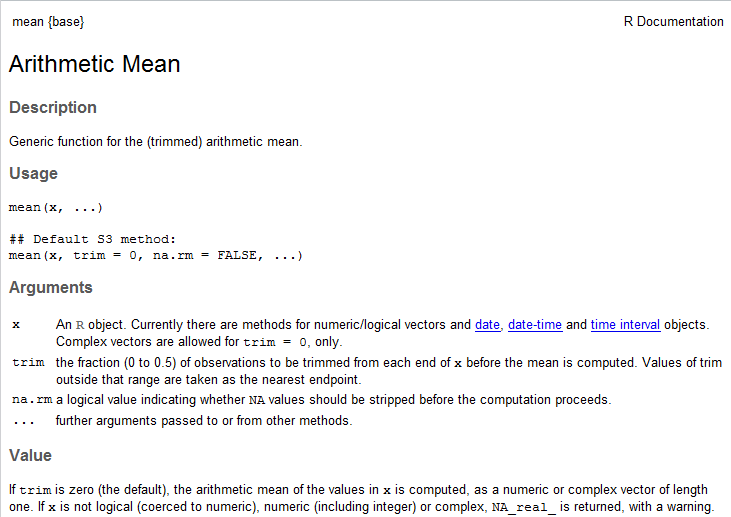
\includegraphics[width = 5in]{mean_help.png}
\end{figure}
\FloatBarrier
Notice the ellipsis (\texttt{...}) after the comma in the \texttt{Usage} section. The ellipsis means that other arguments can be passed to the function. For example, the \texttt{na.rm} argument we covered earlier. However, there are other arguments that we will not cover, and therefore it is best to take on faith that the ellipsis argument will handle whatever it needs to.

\chapter{Descriptive Statistics}
Thus far, all we have covered are functions relating to data and data manipulation. However, R also has many powerful functions for doing statistics. Many of these must be downloaded from other packages, but many can also be found in the base R package that is automatically installed and loaded for you.

\section{Simple Descriptives}
Quick view of functions:
\begin{tabular}{c|l}
Summary Measure & R (base) \\
\hline
mean & \texttt{mean()}\\
Median & \texttt{median()}\\
SD and Variance & \texttt{sd()}, \texttt{var()}\\
Min and Max & \texttt{min()}, \texttt{max()}
\end{tabular}
\\
In R, we have a few different options to find simple descriptive statistics. In the base package, we can get a good summary of the data by using the \texttt{summary()} function. We can also get simple descriptive statistics using the \texttt{mean(), sd(), var()} and other functions. Many of the other simple functions (\texttt{sum} - compute a sum, \texttt{dim} - return the dimensions of an object) operate in a similar way.

\section{Other Descriptives}
For some complex descriptive statistics, as well as some statistical tests and plotting, we suggest using the \texttt{uwIntroStats} package, as well as some other packages besides base R. For a full look at any of these packages, look up their documentation and see which functions they provide. 

\chapter{Chi-square Test}
Quick view of functions:
\begin{tabular}{c}
 R (base)\\
\hline
\texttt{chisq.test()}\\
\end{tabular}\\
\\
The base R function \texttt{chisq.test} performs the chi-squared test on tables, matrices, and vectors. However, in order to calculate Odds Ratios, Risk Ratios, or other statistics (for example the likelihood ratio, Mantel-Haenszel statistic, and others) you must use other functions developed for different R packages and piece the information together. For example, the \texttt{Exact} package contains functions for calculating Odds and Risk ratios.

\chapter{Plots}

\section{Boxplots}
Quick view of functions:
\begin{tabular}{c}
R (base) \\
\hline
\texttt{boxplot()}
\end{tabular}\\
\\
Boxplots can be quite controversial as a descriptive plot of the data. Firstly, the population quartiles are most often not the parameters of interest and so the box plot may not provide meaningful insight in answering a scientific question. The definition of an `outlier" as defined by lying 1.5 $\times$ the interquartile range away is indeed arbitrary; we don't have a good sense of what would be a better replacement. In base R, this is precisely how the outliers are calculated. The minimum, median, IQR, and maximum are also displayed.



\section{Histograms}
Quick view of functions:
\begin{tabular}{c}
R (base) \\
\hline
\texttt{hist()}
\end{tabular}\\
\\
In R, the default for plots is to not label the axes. So if we want our plots to look presentable, we must label the axes. Thus we use the \texttt{ylab} and \texttt{xlab} arguments to apply a y and x-axis label to the plot. The \texttt{breaks} command allows us to enter the number of bins we want displayed on the histogram.

\section{Scatterplots}
Quick view of functions:
\begin{tabular}{c}
R (base) \\
\hline
\texttt{plot()}
\end{tabular}\\
\\
The base R version of the scatterplot takes an \texttt{x} and a \texttt{y} variable (which must be of the same length) and plots the points as specified by these coordinates. If you wish to have least squares lines or other additions to the plot, you must use the \texttt{abline()} function. 

\chapter{Correlations}
Quick view of functions:
\begin{tabular}{c}
R (base)\\
\hline
\texttt{cor()} - correlation\\
\texttt{cov()} - covariance  
  \end{tabular}\\
\\

\section{Pairwise Correlations}

\chapter{Cumulative Distribution Functions}
Say we calculate a test statistic (z-score, t-statistic, chi-squared statistic) and want to find the p-value. Recall that for a p-value we want to find the probability of values at least as extreme as our value. The function for a z-score (defined on the normal distribution) is \texttt{1-pnorm(1)}. Similar functions - \texttt{p} followed by the name of the distribution - can be found for many of the probability distributions.

\chapter{One-Sample Inference}

\section{The one-sample t-test}
Quick view of functions:
\begin{tabular}{c}
R (base)\\
\hline
\texttt{t.test()}\\
\end{tabular}\\
\\

R has a default function called \texttt{t.test} which performs a one-sample t-test. 
\chapter{Two-Sample Inference}

\section{The two-sample t-test}


\chapter{Linear Regression}
Quick view of functions:
\begin{tabular}{c}
R (base) \\
\hline
\texttt{lm()}\\
\end{tabular}\\
\\

\chapter{Regression on Functionals other than the Mean}
Quick view of functions:
\begin{tabular}{cc|l}
Functional & Name & R (base)\\
\hline
Odds & Logistic & \texttt{glm(family = binomial)}\\
Rate & Poisson & \texttt{glm(family = poisson)}\\
Hazard & Proportional Hazards & \texttt{coxph()}\\
\end{tabular}\\
\\
The functionals listed above are listed above regress on the functional listed in the name of the function. They produce similar output to those in the previous chapter. 

\chapter{Graphical User Interfaces}
Often, it is more convenient to use a graphical user interface (GUI) rather than use R from the command line. R comes pre-loaded with a GUI. Typing functions in the GUI is exactly the same as typing in the command line, but the GUI presents everything in a way that is easier to understand and follow. GUIs also provide buttons and tabs that do some useful tasks for the user.
\section{The Basic R GUI}
When you install R, it will usually ask to install a shortcut for R on your desktop. If you use the R application this way (or from the Start menu for Windows users or from the Applications folder for Macintosh users) the basic R GUI will open up. It looks something like this:
  \newline
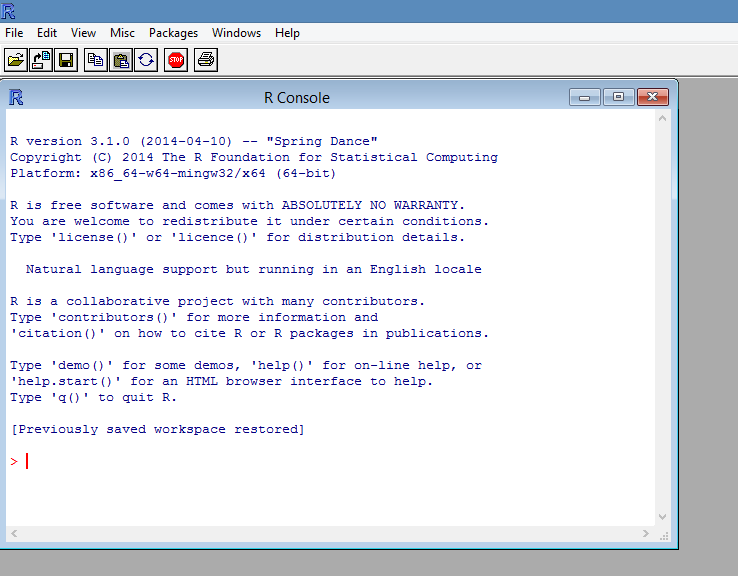
\includegraphics[width=2in, height=2in]{rgui_basic.png}
\newline 
The tabs at the top all have fairly self explanatory functions, from creating and saving scripts to loading packages. The scripts and any plots that are generated appear in the grey space in the GUI window. The main console opens up and is titled ``R Console''. 
\section{RStudio}
There are many other GUIs for R, but a very intuitive one is called RStudio. It can be downloded from www.rstudio.com for free. Before you download RStudio, you must have a version of R downloaded already. You must tell RStudio when you are initially setting it up which version of R to look to. RStudio has all of the same functionality as the basic R GUI, but adds nice features such as the ``Import Dataset'' button which, given the path to a file on your computer or on the internet, downloads and formats the data for you.

\end{document}
